\documentclass[UTF8]{article}
\author {Zhenyu Fan}
\title {My First Latex document}
\usepackage{ctex}
\usepackage{amsmath}
\usepackage{amssymb}
\usepackage{color}
\usepackage{amsmath}
\usepackage{graphicx}
\usepackage{listings} %插入代码
\usepackage{xcolor} %代码高亮

\lstset{language=r,
  basicstyle=\ttfamily,
  keywordstyle=\color{blue},
  commentstyle=\color{darkgreen},
  stringstyle=\color{red}}
\begin{document}
\maketitle
  \paragraph{Question One:}
  Suppose you are a consultant to the local tourism authority and the CEO
  of the authority would like to know whether a family’s annual expenditure on
  recreation is related to their annual income. In addition, if there is a
  relationship, he would like you to build a statistical model which quantifies
  the relationship between the two variables. A data set consisting of a random
  sample of 8 families, collected last year, is available to help you with the
  assessment.
  \\
  \begin{tabular}{ccc}
    \hline
      Y:Expenditure(\$1k) & X: Income(\$1k)\\
    \hline
      2.35 & 52.0\\
      4.95 & 66.0\\
      3.10 & 44.5\\
      .50 & 37.7\\
      5.11 & 73.5\\
      3.10 & 37.5\\
      2.90 & 56.7\\
      1.75 & 35.6\\
    \hline
  \end{tabular}

  (a) Fit a linear regression $y = \beta_0 + \beta_1 x + \epsilon$ on the data.
  Denote $b_0$ and $b_1$ as the least square point estimations of $\beta_0$ and $\beta_1$.
  Calculate $SS_{xx}$, $SS_{yy}$, and $SS_{xy}$, and then calculate $b_0$ and $b_1$.
  \\
  (b) Give an interpretation of each: $b_0$ and $b_1$ \\
  \\
  \paragraph{\color{red}{Answer:}}
  \\
  (a) This is the R code:
  \\
  \begin{lstlisting}[language ={R}]
  x <- c(52.0,66.0,44.5,37.7,73.5,37.5,56.7,35.6)
  y <- c(2.35,4.95,3.10,2.50,5.11,3.10,2.90,1.75)

  sum_xs <- sum(x^2)
  sum_1 <- (sum(x))^2
  SS_xx <- sum_xs - (b / length(x))

  sum_xy <- sum(x * y)
  sum_2 <- sum(x) * sum(y)
  SS_xy <- sum_xy - (sum_2 / 8)

  b_1 <- SS_xy / SS_xx
  b_0 <- mean(y) - b_1 * mean(x)

  sum_ys <- sum(y^2)
  sum_3 <- (sum(y))^2
  SS_yy <- sum_ys - (sum_3 / 8)

  # > SS_xx
  # [1] 21448.17
  # > SS_yy
  # [1] 10.1324
  # > SS_xy
  # [1] 100.395
  \end{lstlisting}
  (b) We can get the $y = -0,39495 + 0,07167187x + \epsion$ \ When $x = 60$, $y = 3.905362$ \\
  So, we can get these information: if a family's income is \$60,000, the expenditure
  is about \$3910 .

  \\
  \paragraph{Question Two:}
    Consider the regression model
    $$ y = \beta_0 + \beta_1 + \epsilon $$
    to fit a data set $\{(x_i, y_i)\}$, that is
    $$ \y_i = \beta_0 + \beta_1 x_i + \epsilon_i, i = 1, \dots n $$\\
    Answer the following questions:
    (a) Give an explanation for $y, x, β_0$ and $β_1$ in model (1). \\
    (b) For obtaining the least square estimates and performing the hypothesis test, what are the assumptions
    for model (2)? \\
    (c) Prove that the point $\(\overline{x}, \overline{y}$ is on the regression
    line $\hat{y} = \hat{\beta_0} + {beta_1}x$, where$\overline{X} = \frac{1}{n}\sum^n_{i=1} x_i$ and $\overline{y} = \frac{1}{n} \sum^n_{i=1} y_i$.
    $\hat{\beta_0}$ and $\hat{\beta_1}$ are the estimates of $beta_0$ and $\beta_1$, respectively.
    \\

  \paragraph{\color{red}{Answer:}}
    \subparagraph{(a)}
      $x$ is the independent variable and $y$ is the dependent variable; \\
      $\beta_0$ is a peremiter that not influenced by the $x$ but by other variable; \\
      $\beta_1$ means that if $x$ increase 1, then the value may increase $y$ values.
    \subparagraph{(b)}
      We have to assume that $\epsilon_1, \epsilon_2,\dots,\epsilon_i$ are i.i.d, and
      $\epsilon~N(0,\sigma^2)$
  \\

  \paragraph{Question Three}
    Answer the following questions:
  \subparagraph{(a)}
    Who proposed the term "regression?" What is the regression phenomenon?
  \subparagraph{(b)}
    Suppose we want to estimate $\beta_0$ and $\beta_1$ in model (1) (see question 2).
    Explain in words what are the least squares estimate,
    $L_1$ - norm estimate and robust estimate respectively, according to the following formulas:\\
    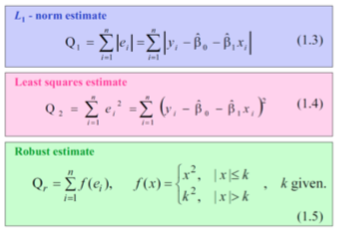
\includegraphics[width = .8\textwidth]{Q3.png} \\
    where $e_i = y_i - \hat{y_i}$, $\hat{y_i} = \hat{\beta_0} + \hat{\beta_1}x_i$.

\paragraph{\color{red}{Answer:}}
  \subparagraph{(a)}
    The term "regression" was coined by Francis Galton in the nineteenth century
    to describe a biological phenomenon. The phenomenon was that the heights of
    descendants of tall ancestors tend to regress down towards a normal average
    (a phenomenon also known as regression toward the mean).
  \subparagraph{(b)}
    The method of least squares is a standard approach in regression analysis to
    approximate the solution of overdetermined systems, i.e., sets of equations in
    which there are more equations than unknowns. "Least squares" means that the
    overall solution minimizes the sum of the squares of the residuals made in the
    results of every single equation.
    \\
    $\mathrm{L}_1 - norm \ estimate$: First we have to sum of the absolute
    values of residuals at all the data points and then we use $\mathrm{L}_1 - norm \ estimate$:
     to minimize them.

\paragraph{Question Four:}
  Let $x_1, \dots, x_n$ be $n$ numbers.

  \subparagraph{(a)}
    Prove:
    \boldmath
    $$
      \sum^n_{i=1}(x_i - \overline{x})^2 ={x'D_nX}
    $$
    where ${x} = (x_1,\dots,x_n)$ and ${D_n = I_n} = \frac{1} 1_n {1'}_n$,
    where $I_n$ is the identical matrix of order $n$ and ${1_n}$ is the n-vertor
    of one's.

  \subparagraph{(b)}
    Prove that ${D_n}$ is a projection matrix with rank $n - 1$
  \subparagraph{(c)}

    Let ${z = D_ny}$, where y is an n-column vector. Show that the sample mean of $\textbf{z}$
    is zero and $z = D_nz$.
  \subparagraph{(d)}

    Prove ${B = \frac{1}{n}1_n{1'}_n}$ is a projection matrix and find its eigenvalues.
\paragraph{Answer:}
  \subparagraph{(a)}
    We can get this equations: \\
    \begin{align*}
      \sum^n_{i=1}(x_i - \overline{x}) &= \sum^n_{i=1}(x_i^2 - 2x_i \overline{x} + \overline{x}^2) \\
      & = \sum^n_{i=1}x_i^2 - 2x_i\sum^n_{i=1}\overline{x} + \sum^n_{i=1} \overline{x}^2 \\
      & = x'x - n\overline{x}^2 \\
      & = x'x - n(\frac{1}{n}1'_nx) \\
      & = x'(1_n -\frac{1}{n}1_n1'_n)x = x'D_nx
    \end{align*}
  \subparagraph{(b)}
  Proof: \\
    \begin{align*}
      D_nD_n &= (I_n -\frac{1}{n}1_n 1'_n)(I_n -\frac{1}{n}1_n 1'_n) \\
             &= I_n \frac{2}{n}1_n1'_n +\frac{1}{n^2}1_n1'_n1_n1'_n \\
      D'_n   &= (I_n - \frac{1}{n}1_n1'_n) = I_n - \frac{1}{n}1_n1'_n = D_n
    \end{align*}
  We can notice that $Rank(A) = Trace(A) = n - \frac{1}{n} \times n = n - 1$ \\
  That means, $D_n$ is a projection matrix and its rank is: $n - 1$
  \subparagraph{(c)}
    The sample mean of $z$:
    \begin{align*}
      z &= D_ny =
      \begin{bmatrix}
        1-\frac{1}{n} & -\frac{1}{n} & \dots &-\frac{1}{n} \\
        -\frac{1}{n} & 1-\frac{1}{n} & \dots & -\frac{1}{n} \\
        \vdots & \vdots & \ddots & \vdots \\
        -\frac{1}{n} & -\frac{1}{n} &\dots & 1-\frac{1}{n} \\
      \end{bmatrix}
       +
      \begin{bmatrix}
        y_1 \\
        y_2 \\
        \ddots \\
        y_n \\
      \end{bmatrix} =
      \begin{bmatrix}
        (1-\frac{1}{n})y_1 & ()-\frac{1}{n})y_2 & \dots & -\frac{1}{n}y_n \\
        -\frac{1}{n}y_1 & (1-\frac{1}{n})y_2 & \dots & -\frac{1}{n}y_n  \\
        \vdots & \vdots & \ddots & \vdots \\
        -\frac{1}{n}y_1 & -\frac{1}{n}y_2 &\dots & 1-\frac{1}{n}y_n  \\
      \end{bmatrix}
    \end{align*}
    we can get the mean by using sum values of $z$ and divided by $n$:
    \\
    $\overline{z} = \frac{(1-n \times \frac{1}{n}) y_1 + (1-n \times \frac{1}{n} y_2 + \dots + (1-n \times \frac{1}{n} y_n )}{n} = 0$
    \\
    \\
    $D_nz =
    \begin{bmatrix}
      (1-\frac{1}{n})y_1 & ()-\frac{1}{n})y_2 & \dots & -\frac{1}{n}y_n \\
      -\frac{1}{n}y_1 & (1-\frac{1}{n})y_2 & \dots & -\frac{1}{n}y_n  \\
      \vdots & \vdots & \ddots & \vdots \\
      -\frac{1}{n}y_1 & -\frac{1}{n}y_2 &\dots & 1-\frac{1}{n}y_n  \\
    \end{bmatrix}
    = z $
  \subparagraph{(d)}
    \begin{align*}
        B'B &= \frac{1}{n^2} 1_n 1'_n1_n1_n = \frac{1}{n^2}(n1_n1'_n) = \frac{1}{n}1_n1'_n = B \\
        B' &= \frac{1}{n} (1_n1'_n)' = \frac{1}{n} 1_n1'_n = B \\
        det(B - \lambda I_n) &=
        \begin{bmatrix}
          \frac{1}{n} - \lambda & \frac{1}{n} & \dots & \frac{1}{n} \\
          \frac{1}{n} = \frac{1}{n} - \lambda & \dots & \frac{1}{n} \\
          \vdots & \vdots & \ddots & \vdots \\
          \frac{1}{n} & \frac{1}{n} & \dots & \frac{1}{n} - \lambda \\
        \end{bmatrix} \\
        \Rightarrow \lambda &= \frac{1}{n}
    \end{align*}
    It is noticeable that $B = \frac{1}1_n1'_n$ is the projection matrix and
    its eignvalue is $\frac{1}{n}$

\end{document}
